\subsection{Review Project Setup}
This chapter reflects on the initial setup and organization of our project.

\subsubsection{Initial Situation}
Our project began with an in-depth analysis of the provided functional and non-functional requirements.
We used the initial project description as a guiding framework and scheduled a meeting with our coach, Dr. Simon Kramer, to clarify any ambiguities.
This analysis led to several key insights:
\begin{itemize}
    \item The application must be platform-independent and developed in Java.
    \item The code should be minimalistic, modular, and self-explanatory.
    \item A public repository is required for code availability.
    \item We depend on external resources like Archive Today and Apache PDFBox.
    \item A console application is preferred, eliminating the need for a graphical interface.
\end{itemize}

This systematic approach allowed us to create a modular and extendable codebase.
When the integration of the Wayback Machine was later introduced as a requirement by our stakeholder, our well-structured codebase enabled us to agilely accommodate this new feature.
This addition was assessed to ensure it added value to the project and didn't become a blocker, demonstrating the effectiveness of our initial analysis and flexible project approach.

\subsubsection{Subject analysis}
In our subject analysis, we thoroughly researched necessary external resources, focusing on Archive Today and the Wayback Machine.
Our investigation included their automation interfaces, REST API support, and potential challenges such as Captcha and login requirements.
We also ensured these resources were compatible with our FLOSS licensing requirement.
This study allowed us to design an initial user interaction model and provided a clear roadmap for our application's development, facilitating a smooth transition into the coding phase.

\subsubsection{Stakeholder(-Management)}
Our stakeholder management focused on effective communication with our primary stakeholder, Dr. Simon Kramer.
We efficiently addressed any uncertainties by scheduling regular meetings with Dr. Kramer, utilizing our designated Project 1 timeslot.
This approach allowed for straightforward and effective resolution of questions and alignment of project deliverables.

\subsubsection{Organisation}
Our team's organization was based on agile principles, with scheduled Monday and Friday meetings serving as our Scrum events.
These structured sessions were complemented by self-organized meetings among team members as needed, facilitating code reviews, quick resolution of questions, or addressing any issues.
This agile approach ensured effective communication and collaboration, which was vital for the project's smooth progression.

\subsubsection{Installations}
For our project installations, we established a GitHub repository and a Jira project on Atlassian.net, ensuring efficient collaboration.
Our first week involved defining objectives and creating epics in Jira.
We also updated our IDEs and installed the latest Java version for consistency.
Reflecting back, an early setup of a basic code structure would have been beneficial, potentially minimizing the need for later refactoring.

\subsection{Review}
This chapter provides a review of our project, discussing the management of our sprints and backlogs, and our progress towards achieving our product goal.

\subsubsection{Product goal}
Achieving the product goal for the URL Archiver application was a journey of iterative development and unwavering commitment to our goals.
We successfully developed a platform-independent, CLI-based Java application that met all the specified functionalities, including efficient URL extraction, archiving options and CSV file generation.
The application adheres to FLOSS licensing, ensuring open-source availability.
Accompanying this, we created detailed user manuals, installation instructions and thorough software documentation.
Our code is characterised by minimalism and modularity, with self-explanatory sections that underline our commitment to quality and maintainability.

\subsubsection{Sprint goals}
Throughout the sprints, we've rigorously set our goals in alignment with the SMART criteria, ensuring clarity and measurable targets.
From the foundational work of implementing a robust input handler in Sprint 1 to enhancing system stability in Sprint 4, each goal was carefully crafted and successfully achieved.
Sprint 5's focus on asynchronous archiving refined our application's functionality, while Sprint 6's emphasis on design and documentation prepared us for the final review.
This structured approach to goal-setting has been instrumental in our consistent delivery of sprint objectives.

\subsubsection{Delimitation}
The delimitation in our project was implicitly conducted through disciplined backlog management and sprint planning.
We confined our efforts to the most critical features, implicitly setting boundaries that guided our development focus.
This implicit delimitation allowed us to concentrate resources on the highest priority tasks, ensuring the project’s scope remained tightly aligned with our key objectives.
While a formal delimitation review was not performed, our adherence to Agile principles effectively served the same purpose, keeping the project streamlined and on target.

\subsubsection{Delivery objects}
We successfully developed a platform-independent Java application that follows the principles of FLOSS.
The application includes a command-line interface for ease of use, can process various file inputs, has URL extraction and archiving functionalities, and generates a CSV file documenting the archived URLs.
In addition, we provided user manuals, installation scripts, and software documentation to improve user experience and understanding.
Our attention to detail and commitment to our goals throughout the project's lifecycle resulted in successfully meeting our delivery objectives.

\subsubsection{Product Backlog}
Our product backlog management was an exercise in adaptability and strategic foresight.
In collaboration with our stakeholder, we regularly assessed and updated our backlog, ensuring it remained relevant and reflective of current project needs.
This iterative process, led by the Product Owner, involved introducing new user stories and de-prioritizing or removing those that had lost their relevance.
Our focus was on high-priority tasks that directly contributed to achieving the product goal, while medium and low-priority items were cataloged for potential future development.
This approach maintained a balance between addressing immediate project requirements and envisioning future enhancements.
The careful maintenance of the backlog provided a clear roadmap for our efforts, crucial for the effectiveness of our sprint reviews and overall project progress.

\subsubsection{Sprint Backlogs}
Throughout the sprints, our team demonstrated a commendable ability to effectively manage and complete the sprint backlogs.
We consistently improved our workload management with each sprint, adapting our strategies based on previous experiences.
There was only one instance of user stories being carried over to the next sprint, reflecting our overall planning efficiency and responsiveness to unforeseen challenges.
The velocity report illustrates this progress, with an upward trend in completed story points, underlining our growing proficiency in sprint management.
\begin{figure}[h!]
    \centering
    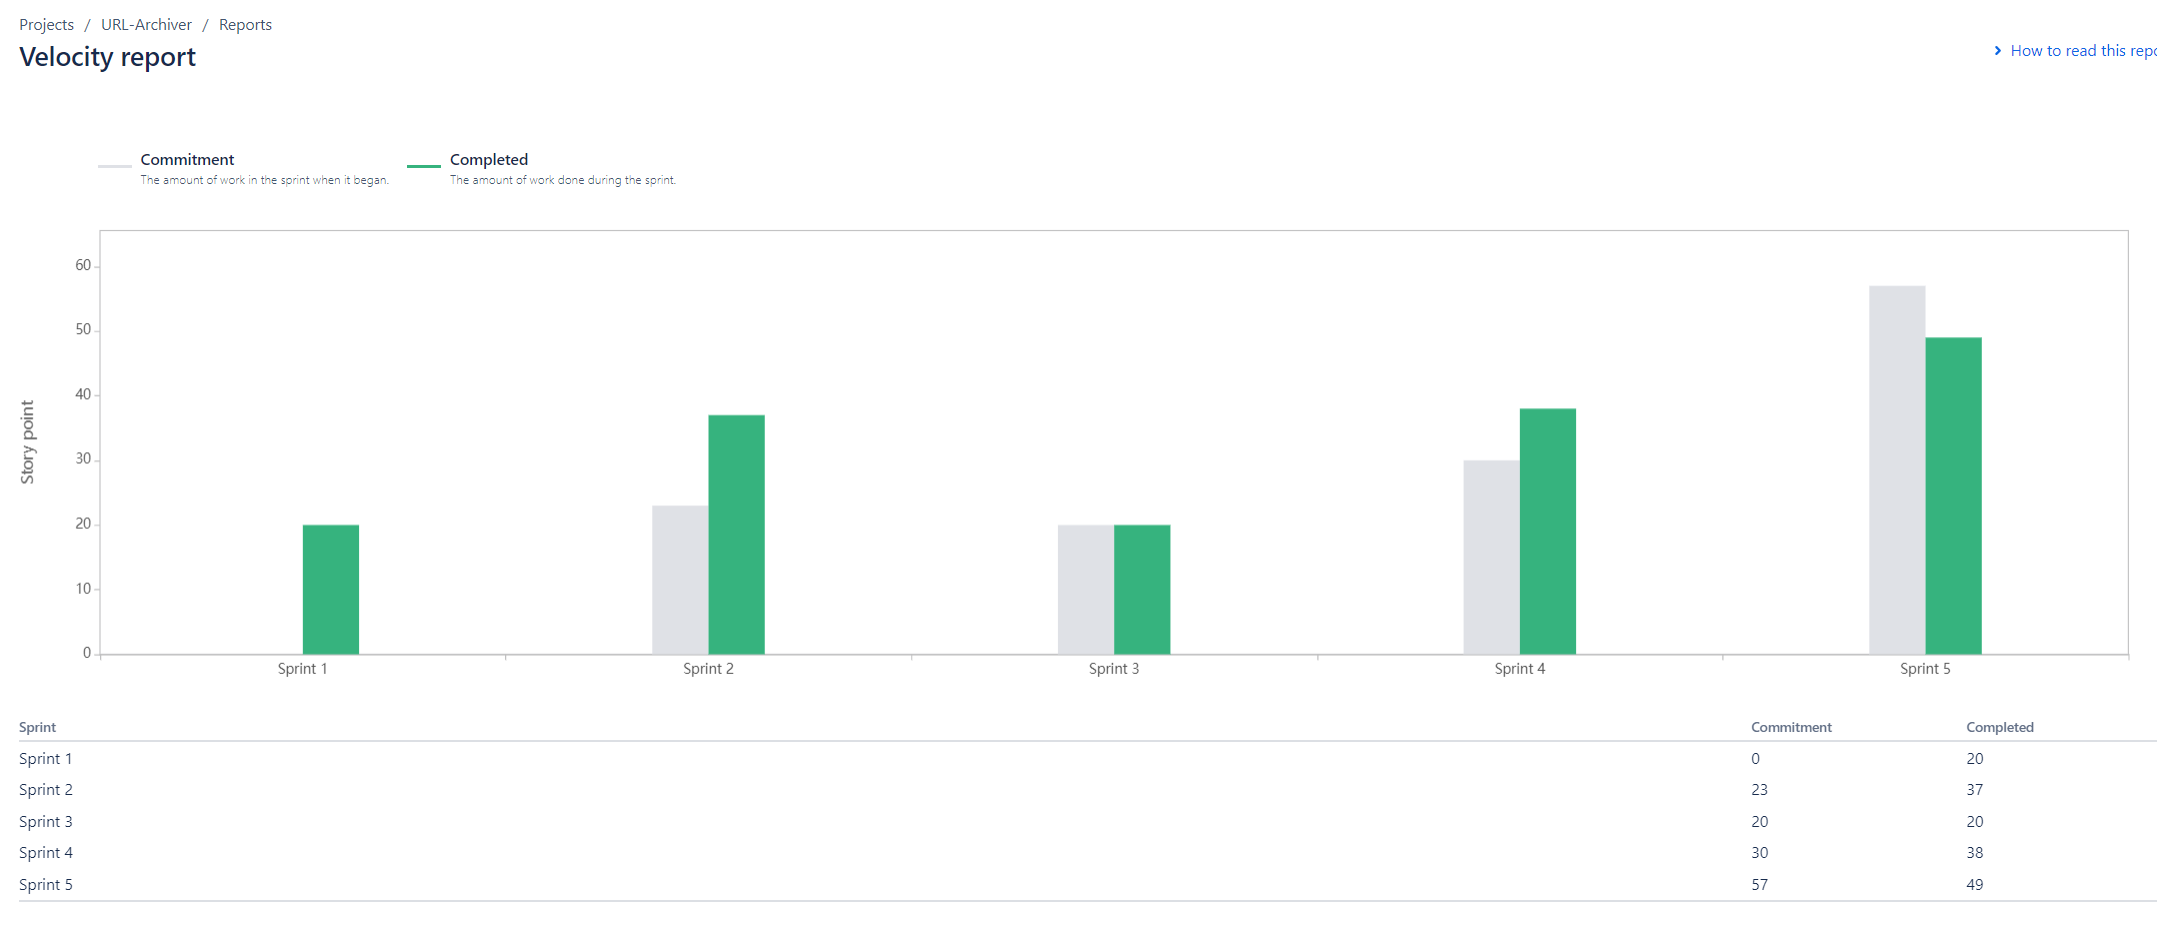
\includegraphics[width=1\textwidth]{pictures/Scrum/velocity_report}
    \caption{Velocity Report}
    \label{fig:velocity_report}
\end{figure}

\subsection{Retrospective I: Scrum Method}
This chapter reflects on the distribution and implementation of Scrum roles as previously described.
It also considers our insights from Scrum Events and Scrum Artifacts.

\subsubsection{Scrum Roles}
Nicolin fulfilled the role of Product Owner exceptionally well.
He consistently maintained and prioritized the Product Backlog.
Moreover, he ensured we were in close communication with our customer, Mr. Kramer, guaranteeing that stakeholder requirements were discussed and incorporated.
This was instrumental in the business success of the product being developed.

Abidin, as Scrum Master, executed his responsibilities with diligence, evident in the efficient Scrum operation of the team.
Acting as a liaison between the Product Owner and the Developers, any questions regarding the agile methodology were promptly clarified.
Additionally, obstacles beyond the team's capacity were resolved with the involvement of our coaches.

Kilian held the role of developer and played a key role in shaping the product.
As there were only three of us in the project team, Abidin and Nicolin also contributed to the technical development.
Our goal to satisfy our client, Mr. Simon Kramer, was achieved through the early and continuous delivery of our software.
This ensured the software developed matched Mr. Kramer's vision and requirements.
Moreover, we were able to implement new requirements during the project, as clearly demonstrated by integrating the Wayback Machine.
Throughout the project, we maintained self-organization, a consistent pace, reflection, and expeditious work.

\subsubsection{Scrum Events}

\paragraph{Sprint}
Our two-week sprint cycles have been effective in balancing workload and facilitating regular feedback.
Setting SMART goals for each sprint provided us with a clear and focused direction and contributed significantly to our team's progress.
Although we occasionally faced challenges in estimating workload, these instances offered valuable lessons in capacity planning.
Exploring more precise estimation techniques could improve our ability to align tasks with our team's capacity, building on our already solid sprint planning process.

\paragraph{Sprint Planning}
Sprint planning was a strong point for our team, particularly with the upfront estimation of user stories and prioritization based on business value and team velocity.
We ensured that the most impactful tasks were addressed each sprint.
Encountering larger-than-expected user stories at times provided learning opportunities for better task evaluation.
A more comprehensive review process for estimating user stories could strengthen our sprint planning further.

\paragraph{Daily Scrum}
Adjusting to bi-weekly meetings complemented our part-time work schedules and kept our team communication robust.
Using Microsoft Teams for meetings added flexibility and convenience.
While the format sometimes delayed the addressing of immediate issues, it generally promoted focused and efficient discussions.
A mid-week check-in could enhance our responsiveness without burdening the team's schedule.

\paragraph{Sprint Review}
Our sprint reviews were invaluable, offering objective evaluations that kept product increments in line with customer needs and expectations.
Responding to customer feedback, though sometimes challenging, was a dynamic learning opportunity that led to significant product enhancements.
More frequent reviews during the sprint could make the feedback integration process even smoother.

\paragraph{Sprint Retrospective}
The sprint retrospectives were characterized by constructive, open discussions that effectively pinpointed our successes and growth areas.
These sessions were instrumental in fostering a culture of continuous improvement, with actionable steps consistently identified to enhance team processes.
While implementing these improvements took effort, the retrospectives were central to our team's development and unity.
A structured follow-up mechanism for retrospective suggestions could maximize these sessions' impact.

Although we attempted to provide each other with honest and constructive feedback, we realised that it can be challenging to do so.
This is often due to fear of the recipient's reaction.
However, we believe that with time, giving feedback will become easier for a team that has worked together for an extended period.

\subsubsection{Scrum Artifacts}

\paragraph{Product Backlog}
The Product Backlog was a dynamic, well-organized tool that effectively captured our project's requirements and priorities.
Regular updates and refinements ensured it remained in sync with our evolving project goals and customer needs.
Clear categorization and prioritization of items significantly aided our planning and decision-making.
We are considering incorporating more frequent stakeholder feedback sessions to ensure that the backlog continues to reflect the most current and relevant project needs.

\paragraph{Sprint Backlog}
Our Sprint Backlog was used effectively to map out user stories, providing a clear outline of the sprint goals.
Generally, we managed without creating detailed tasks for each story, favoring a broader view for simplicity and clarity.
Introducing specific tasks for user stories in future sprints could improve granularity and task management.
This approach could enhance tracking and aid in early obstacle identification.

\paragraph{Product Increment}
Our approach to product increments has highlighted our team's dedication to delivering high-quality results at the end of each sprint.
The increments met the set criteria and client expectations, showcasing our ability to effectively transform backlog items into tangible, valuable product features.
Regular reviews and refinements ensured alignment with project goals and customer needs.


\subsection{Retrospektive II: Tools/Instruments}

\subsubsection{Insights tool use}
During the project, we used various tools that were essential to our success.
In this section, we will discuss these tools and our experiences with them.

\paragraph{Java}
Java, our chosen primary programming language, facilitated a smooth development process due to the team's pre-existing knowledge.
This familiarity allowed us to focus on delivering a high-quality application efficiently.

\paragraph{Maven}
Maven's role in our project was critical, handling compilation, dependency management, and the building process.
Our prior experience with Maven enabled its seamless integration into our workflow, contributing to a smooth development cycle.

\paragraph{JUnit 5}
JUnit 5 played a pivotal role in our testing framework, guaranteeing the stability and reliability of our application, especially following code refactoring activities, thus ensuring the integrity of our application's logic.

\paragraph{JetBrains IntelliJ IDEA}
The selection of IntelliJ IDEA as our integrated development environment provided an array of tools that streamlined our development processes, enhancing productivity, and facilitating a high level of code quality.

\paragraph{GitHub}
GitHub was the backbone of our version control system, offering a robust platform for collaborative code management.
It enabled efficient teamwork and was essential in maintaining a consistent codebase.

\paragraph{Atlassian Jira}
Atlassian Jira was a cornerstone of our project management, enabling us to track progress, manage priorities, and streamline our workflow effectively, proving itself as an invaluable asset to our project organization.

\paragraph{LaTeX}
LaTeX was used for creating our project documentation and presentations.
Despite initial challenges due to varying levels of experience within the team, it ultimately enabled us to produce professional and consistent documentation.

\subsubsection{Communication}

\paragraph{Microsoft Teams}
With Microsoft Teams, we were able to streamline our communication, enabling an effective platform for meetings and Scrum events that fostered rapid problem resolution and team agility.
The platform's flexibility and immediacy were crucial to our effective problem-solving process.

\paragraph{Email and BigBlueButton}
For external communications, particularly with coaches, we used email for asynchronous exchanges and BigBlueButton for real-time video conferencing, ensuring clear and direct dialogue with our stakeholders.

\subsubsection{Controlling}

\paragraph{Atlassian Jira}
Jira served as the central control tool for our project, providing a comprehensive overview of project status and task distribution.
It facilitated clear categorisation and prioritisation of tasks, thereby enhancing our workflow and project management.

\paragraph{Burndown Charts}
We utilized Burndown Charts to monitor our sprint efficiency and to inform future sprint planning.
This allowed for a balanced workload management and realistic goal-setting based on our team's velocity and past performance.


\subsection{Lessons learned}

\subsubsection{Team}

\subsubsection{Nicolin Dora}
Developing and managing my first software project from scratch was a great experience.
However, working with SCRUM was challenging as we could only work on weekends or evenings due to part-time study.
This made it difficult to use SCRUM effectively, and planning and report preparation took almost as much time as product development.
In principle, SCRUM is a useful method as it allows for easy tracking of project progress.
However, the students could have been given more freedom in this project to simplify the method.

I enjoyed the teamwork and appreciated the goal-oriented approach.
It was interesting to balance the different demands on quality.
Mr. Kramer and Mr. Helbling were always available to answer questions, which made collaboration easier.
For future projects, I plan to use a slimmed-down version of SCRUM, depending on the complexity of the project.
I am determined to improve my planning and communication within the team right from the start.

\subsubsection{Abidin Vejseli}
Project 1 has been an enriching yet demanding journey, requiring meticulous time management and organization from my side.
The Scrum methodology, which I believe our team adapted effectively, and the complexities of part-time study contributed to this challenge.
Personally, I felt the initial module introduction was rather lengthy and could be condensed to the essential material.
It was unfortunate not to have both coaches at the presentation, which was an aspect that I missed.

Working within the team was a positive experience, and I'm proud of how we distributed the workload, ensuring valuable learning for everyone.
The interaction with our coaches was a highlight, their readiness to assist was something I greatly appreciated.
For the next project, I aim to start and ideally complete my user stories during the first half of the sprint.

\subsubsection{Killian Wampfler}
For me, Project 1 was a great refresher for my programming skills and software development techniques.
As I already use the Scrum method in my company, this part wasn't new to me.
However, it was interesting to use the Scrum method in such a small team (3 people).
Also, the team worked really well together and I think we could all learn something from this project.

Personally, I learned two things from this project.
First, my unit tests have a lot of room for improvement (in quality and quantity).
And more importantly, my git commit messages weren't the norm.
Because of this, our git repository doesn't look consistent, and as this project needs to be publicly accessible, this is not desired.

Lastly I really appreciated how much freedom Mr. Kramer gave us and that he always took the time to answer our questions.